% ===================== CHƯƠNG 3: KẾT QUẢ ===========================
\chapter{KẾT QUẢ ĐỀ TÀI VÀ PHÂN TÍCH, ĐÁNH GIÁ, THẢO LUẬN}
\label{ch:ketqua}

Chương này trình bày thiết lập thực nghiệm, kết quả đối sánh giữa EarlyRisk-MOOC và sáu baseline được tái hiện trên cùng giao thức, kết quả thực nghiệm nội tại của khung, và cuối cùng là thảo luận về ý nghĩa lý thuyết--thực tiễn cùng các giới hạn.

\section{Thiết lập thực nghiệm}
\label{sec:thietlap}

\subsection{Bộ dữ liệu và quy trình lọc cohort}

Bộ dữ liệu sử dụng là MOOCCubeX của Yu và cộng sự \cite{Yu2021}, với 3,3 triệu người học và 4.216 khóa học. Quy trình lọc cohort giữ lại các cặp $(i, c)$ có hoạt động thực sự trong 4 tuần đầu và tổng tương tác đạt ngưỡng tối thiểu, cho cohort thực nghiệm gồm 100.409 cặp người học--khóa học. Bảng~\ref{tab:cohort} tóm tắt thống kê chi tiết của cohort.

\begin{table}[H]
\centering
\caption{Thống kê chi tiết cohort thực nghiệm sau khi lọc từ MOOCCubeX}
\label{tab:cohort}
\renewcommand{\arraystretch}{1.25}
\small
\begin{tabularx}{\textwidth}{@{}X r@{}}
\toprule
\textbf{Thuộc tính} & \textbf{Giá trị} \\
\midrule
Tổng số cặp người học--khóa học & 100.409 \\
Số người học duy nhất & 67.824 \\
Số khóa học duy nhất & 421 \\
Số bản ghi sự kiện hành vi (4 tuần) & $\approx$ 8,2 triệu \\
\midrule
\multicolumn{2}{@{}l}{\textit{Phân phối nhãn 5 mức}} \\
\quad Lớp A (hoàn thành rất tốt) & 2,22\% \\
\quad Lớp B (tốt) & 8,12\% \\
\quad Lớp C (trung bình) & 7,69\% \\
\quad Lớp D (đang hoạt động, rủi ro cao) & 64,11\% \\
\quad Lớp E (không hoàn thành / bỏ học) & 17,85\% \\
\midrule
\multicolumn{2}{@{}l}{\textit{Số khóa đã đăng ký của mỗi người học}} \\
\quad Trung bình / trung vị / tối đa & 1,48 / 1 / 17 \\
\quad Số người học có $\geq 2$ khóa & 18.532 (27,3\%) \\
\midrule
\multicolumn{2}{@{}l}{\textit{Số đặc trưng đầu vào}} \\
\quad Đặc trưng hành vi tuần (9 stems $\times$ 4 tuần) & 36 \\
\quad Đặc trưng tĩnh (nhân khẩu, khóa) & 16 \\
\quad Tổng đầu vào (tại W4) & 52 \\
\midrule
Phần cứng & Microsoft Fabric Spark pool \\
Driver & 8 vCPU, 56 GB RAM, không GPU \\
\bottomrule
\end{tabularx}
\end{table}

Phân phối nhãn cho thấy mức độ mất cân bằng rõ rệt: lớp D chiếm tới 64,11\% trong khi lớp A chỉ chiếm 2,22\%. Đặc điểm này khẳng định tính cần thiết của hàm mất mát tái cân bằng và của việc báo cáo Macro-F1 thay vì chỉ dựa vào Accuracy.

\subsection{Quy tắc gán nhãn và giao thức chia tập}

Quy tắc gán nhãn 5 mức sử dụng một quy tắc lai: neo hai lớp đầu mút A/E theo ngưỡng ngữ nghĩa ($\geq 0{,}9$ cho A; $= 0$ cho E), sau đó chia ba lớp giữa B/C/D theo phân vị của chỉ số tổng hợp $0{,}6 \cdot \text{course\_norm\_score} + 0{,}4 \cdot \text{completion\_rate}$, sao cho không có lớp nào chiếm dưới 1\%. Các đặc trưng tổng hợp toàn bộ 4 tuần bị loại khỏi vector đầu vào để tránh rò rỉ thông tin từ nhãn vào đặc trưng. Giao thức chia tập là phân tầng theo nhãn 5 lớp với tỷ lệ 8:1:1 ở mức cặp $(i, c)$, hạt giống ngẫu nhiên cố định 42. Hạ tầng ETL dùng Apache Spark \cite{Zaharia2016}; huấn luyện mô hình chạy trên \texttt{pandas}/\texttt{scikit-learn}/\texttt{PyTorch} trong cùng môi trường để bảo đảm khả năng đối sánh công bằng.

\subsection{Tái hiện sáu baseline trên cùng giao thức}

Sáu công trình baseline được tái hiện trên cùng giao thức: cùng cohort 100.409 cặp, cùng nhãn 5 mức, cùng split 8:1:1, cùng phần cứng. Bảng~\ref{tab:baseline} liệt kê chi tiết các điều chỉnh chính để mỗi baseline tương thích với thiết lập nhãn 5 mức. Mục tiêu của thí nghiệm đối sánh là: (i) đo khoảng cách hiệu năng định lượng giữa các họ phương pháp trên cùng cohort 5 mức; (ii) phân tích cách mỗi họ phản ứng với cửa sổ quan sát; và (iii) định vị EarlyRisk-MOOC trên đường ranh giới Pareto chi phí--hiệu năng.

\begin{table}[H]
\centering
\caption{Chi tiết tái hiện 6 công trình baseline trên cùng giao thức của EarlyRisk-MOOC}
\label{tab:baseline}
\renewcommand{\arraystretch}{1.3}
\footnotesize
\begin{tabularx}{\textwidth}{@{}p{2.8cm} p{3.2cm} X@{}}
\toprule
\textbf{Công trình} & \textbf{Mô hình tái hiện} & \textbf{Điều chỉnh chính} \\
\midrule
Fei \& Yeung 2015 \cite{Fei2015} & RNN, LSTM & Softmax 5 lớp thay sigmoid; nhãn 5 mức thay nhị phân \\
Alamri 2019 \cite{Alamri2019} & RF, AdaBoost, GB, XGBoost & Hai đặc trưng tuần đầu; ánh xạ ngữ nghĩa step\_visits $\rightarrow$ video\_count \\
Xing \& Du 2019 \cite{Xing2019} & Deep MLP 128-64-32 & Làm phẳng đặc trưng thay vì chuỗi (bài gốc dùng MLP) \\
Dass 2021 \cite{Dass2021} & RF ($n=300$) + SHAP & Tính tiến độ theo tuần thay vì theo ngày \\
Basnet 2022 \cite{Basnet2022} & 5 ML + 3 DL (chọn cấu hình tốt nhất theo Macro-F1) & Đầu ra 5 lớp thay vì nhị phân \\
Aouarib 2025 \cite{Aouarib2025} & GA + XGBoost (pop=12, gens=5) & GA với pop nhỏ vì cohort lớn 100k \\
\bottomrule
\end{tabularx}
\end{table}

\subsection{Hạ tầng xử lý dữ liệu lớn và quy trình ETL}

Quy mô của MOOCCubeX -- với khoảng 296 triệu sự kiện hành vi thô -- đặt ra thách thức xử lý dữ liệu lớn mà một máy đơn khó đáp ứng. Luận văn sử dụng Apache Spark \cite{Zaharia2016} làm hạ tầng ETL nhờ khả năng xử lý phân tán và mô hình tính toán trên bộ nhớ. Quy trình ETL gồm ba giai đoạn chính, tương ứng với ba chữ cái E-T-L.

\textit{Giai đoạn trích xuất (Extract).} Nhật ký thô được đọc từ kho lưu trữ, bao gồm các bản ghi sự kiện xem video, thử bài tập và các tương tác khác. Do dữ liệu thô có kích thước lớn và cấu trúc lồng nhau, giai đoạn này tập trung vào việc phân tích cú pháp và làm phẳng các bản ghi thành dạng bảng thuận tiện cho xử lý tiếp theo.

\textit{Giai đoạn biến đổi (Transform).} Đây là giai đoạn phức tạp nhất, thực hiện lọc cohort, tổng hợp sự kiện thành chín đặc trưng hành vi theo tuần, tính toán các đặc trưng tĩnh, và gán nhãn năm mức. Việc tổng hợp theo tuần đòi hỏi các phép nhóm (group-by) và cửa sổ (window function) trên hàng trăm triệu bản ghi, nơi khả năng xử lý phân tán của Spark phát huy hiệu quả rõ rệt. Nguyên tắc chống rò rỉ được thực thi ngay ở giai đoạn này: các đặc trưng của mỗi cửa sổ chỉ tổng hợp dữ liệu đến tuần tương ứng.

\textit{Giai đoạn nạp (Load).} Dữ liệu đã biến đổi được ghi ra định dạng thuận tiện cho giai đoạn huấn luyện mô hình, vốn chạy trên các thư viện Python (\texttt{pandas}, \texttt{scikit-learn}, \texttt{PyTorch}). Việc tách biệt hạ tầng ETL (Spark) khỏi hạ tầng huấn luyện (Python) là một lựa chọn thiết kế có chủ đích: Spark tối ưu cho xử lý dữ liệu lớn theo lô, trong khi các thư viện Python tối ưu cho thực nghiệm mô hình linh hoạt. Thời gian chạy được báo cáo trong các bảng kết quả chỉ tính giai đoạn huấn luyện mô hình, không bao gồm ETL, vì ETL chỉ cần chạy một lần và được chia sẻ cho mọi cấu hình.

Việc mô tả rõ hạ tầng này có hai ý nghĩa. Thứ nhất, nó bảo đảm tính tái lập: người đọc có thể tái dựng quy trình với cùng công cụ. Thứ hai, nó làm rõ rằng khung EarlyRisk-MOOC được thiết kế với khả năng mở rộng quy mô trong tâm trí -- một yếu tố quan trọng khi hướng tới việc mở rộng cohort lên toàn bộ 3,3 triệu người học của MOOCCubeX.

\section{Kết quả đối sánh với sáu baseline}
\label{sec:doisanh}
Bảng~\ref{tab:sosanh} tổng hợp kết quả của 7 hệ thống trên ba cửa sổ về Macro-F1, Accuracy và Runtime.

\begin{table}[H]
\centering
\caption{So sánh định lượng EarlyRisk-MOOC với 6 công trình tái hiện trên MOOCCubeX (nhãn 5 mức, cohort 100.409 cặp, split 8:1:1, seed = 42)}
\label{tab:sosanh}
\renewcommand{\arraystretch}{1.25}
\footnotesize
\begin{tabular}{@{}l ccc ccc ccc@{}}
\toprule
& \multicolumn{3}{c}{\textbf{Macro-F1}} & \multicolumn{3}{c}{\textbf{Accuracy}} & \multicolumn{3}{c}{\textbf{Runtime (s)}} \\
\cmidrule(lr){2-4}\cmidrule(lr){5-7}\cmidrule(lr){8-10}
\textbf{Công trình} & W1 & W2 & W4 & W1 & W2 & W4 & W1 & W2 & W4 \\
\midrule
Alamri \cite{Alamri2019}      & 0,2677 & 0,1646 & 0,1605 & 0,6736 & 0,6417 & 0,6413 & 7,2 & 7,5 & 7,1 \\
Fei \& Yeung \cite{Fei2015}   & 0,5881 & 0,6550 & 0,7214 & 0,7659 & 0,8010 & 0,8560 & 8,4 & 7,9 & 9,4 \\
Xing \& Du \cite{Xing2019}    & 0,6452 & 0,6849 & 0,7430 & 0,7958 & 0,8193 & 0,8497 & 59,2 & 56,3 & 48,1 \\
Basnet \cite{Basnet2022}      & 0,7987 & 0,7966 & 0,7981 & 0,8857 & 0,8876 & 0,8941 & 6,8 & 7,0 & 8,3 \\
Dass \cite{Dass2021}          & 0,8446 & 0,8515 & 0,8562 & 0,9114 & 0,9166 & 0,9210 & 28,3 & 29,4 & 32,1 \\
Aouarib \cite{Aouarib2025}    & 0,8628 & 0,8638 & 0,8658 & 0,9229 & 0,9243 & 0,9311 & 22,7 & 17,0 & 21,3 \\
\textbf{EarlyRisk-MOOC}       & \textbf{0,8460} & \textbf{0,9499} & \textbf{0,9556} & \textbf{0,8963} & \textbf{0,9686} & \textbf{0,9785} & 40,7 & 48,9 & 56,2 \\
\bottomrule
\end{tabular}
\end{table}

EarlyRisk-MOOC đứng đầu ở W2 và W4 về cả Macro-F1 lẫn Accuracy, nhưng \emph{không} đứng đầu tại W1: ở cửa sổ này, Aouarib (GA + XGBoost) đạt Macro-F1 cao hơn (0,8628 so với 0,8460 của EarlyRisk-MOOC). Tại điểm vận hành W2, khoảng cách Macro-F1 với baseline mạnh nhất là $0{,}9499 - 0{,}8638 = 0{,}0861$, tương đương cải thiện tương đối 9,1\%.

Điểm quan trọng nhất của Bảng~\ref{tab:sosanh} là cách các mô hình phản ứng khác nhau trước cửa sổ quan sát. Hai mô hình chuỗi thời gian, Fei \& Yeung và EarlyRisk-MOOC, hưởng lợi rõ rệt khi cửa sổ tăng từ W1 đến W4 -- EarlyRisk-MOOC tăng từ 0,8460 lên 0,9499 rồi 0,9556, tổng cộng $+0{,}1096$. Đáng chú ý, Xing \& Du -- vốn là một mạng MLP làm phẳng đặc trưng chứ không phải mô hình chuỗi (xem Bảng~\ref{tab:baseline}) -- cũng cải thiện đáng kể theo cửa sổ ($+0{,}0978$ từ W1 đến W4), cho thấy lợi ích của cửa sổ dài hơn không đến riêng từ việc dùng bộ trích xuất chuỗi, mà còn phụ thuộc vào việc kiến trúc có thực sự khai thác thêm thông tin theo tuần khi $W$ tăng hay không. Ngược lại, các mô hình trên đặc trưng đã tổng hợp cố định (Aouarib, Basnet, Dass) gần như không đổi, với chênh lệch chỉ 0,0014--0,0116. Kết quả này góp phần trả lời \textbf{RQ1}: cải thiện theo cửa sổ có xu hướng xuất hiện ở các mô hình có khả năng khai thác thêm thông tin theo tuần, trong khi các mô hình dựa trên đặc trưng tổng hợp cố định ít tận dụng được cửa sổ dài hơn; tuy nhiên vì các họ mô hình trong đối sánh này khác nhau đồng thời về cả kiến trúc lẫn biểu diễn đặc trưng đầu vào, kết quả chưa đủ để khẳng định riêng biệt rằng bản thân việc mã hóa tuần tự (sequential encoding) là nguyên nhân duy nhất của cải thiện quan sát được.

\subsection{Phân tích chi phí--hiệu năng theo lát cắt Pareto}

Hình~\ref{fig:pareto} trực quan hóa mặt tiền Pareto giữa Macro-F1 và Runtime ở cửa sổ W2.

\begin{figure}[H]
\centering
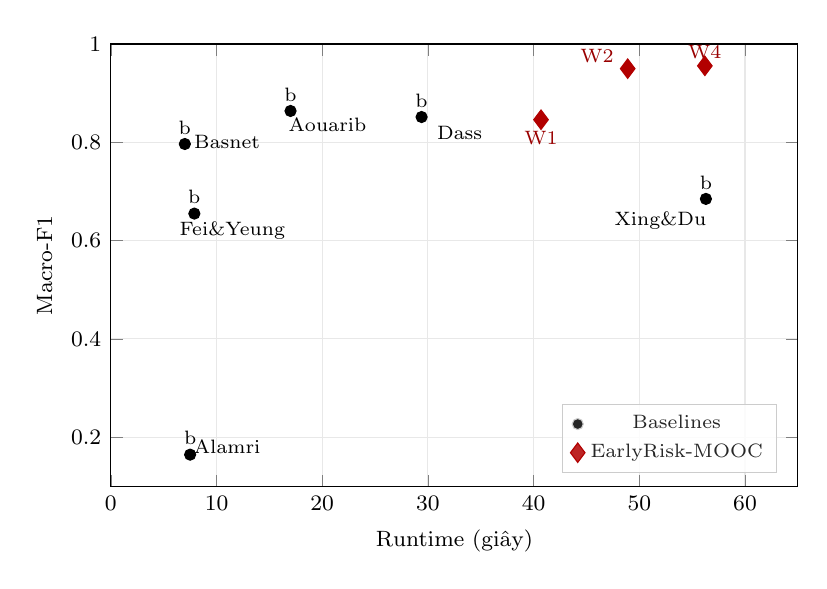
\begin{tikzpicture}
\begin{axis}[
  width=0.85\textwidth, height=7.2cm,
  xlabel={Runtime (giây)}, ylabel={Macro-F1},
  xmin=0, xmax=65, ymin=0.1, ymax=1.0,
  grid=both, grid style={gray!18},
  legend pos=south east, legend style={font=\scriptsize,fill=white,fill opacity=0.85,draw=gray!40},
  tick label style={font=\footnotesize}, label style={font=\footnotesize},
  scatter/classes={
    b={mark=*,draw=black,fill=gray!60},
    e={mark=diamond*,draw=red!70!black,fill=red!70!black,mark size=3.5pt}
  }
]
% baselines at W2
\addplot[only marks,scatter,scatter src=explicit symbolic,nodes near coords,
  point meta=explicit symbolic,
  every node near coord/.append style={font=\scriptsize,anchor=south}]
  coordinates {
    (7.5,0.1646)[b]
    (7.9,0.6550)[b]
    (56.3,0.6849)[b]
    (7.0,0.7966)[b]
    (29.4,0.8515)[b]
    (17.0,0.8638)[b]
  };
% labels for baselines
\node[font=\scriptsize] at (axis cs:11,0.18) {Alamri};
\node[font=\scriptsize] at (axis cs:11.5,0.62) {Fei\&Yeung};
\node[font=\scriptsize] at (axis cs:52,0.64) {Xing\&Du};
\node[font=\scriptsize] at (axis cs:11,0.80) {Basnet};
\node[font=\scriptsize] at (axis cs:33,0.82) {Dass};
\node[font=\scriptsize] at (axis cs:20.5,0.835) {Aouarib};
% EarlyRisk-MOOC at W1/W2/W4
\addplot[only marks,mark=diamond*,red!70!black,mark size=3.5pt]
  coordinates {(40.7,0.8460) (48.9,0.9499) (56.2,0.9556)};
\node[font=\scriptsize,red!60!black] at (axis cs:40.7,0.81) {W1};
\node[font=\scriptsize,red!60!black] at (axis cs:46,0.975) {W2};
\node[font=\scriptsize,red!60!black] at (axis cs:56.2,0.985) {W4};
\legend{Baselines, EarlyRisk-MOOC}
\end{axis}
\end{tikzpicture}
\caption{Mặt tiền Pareto giữa Macro-F1 và Runtime (giây) ở cửa sổ W2. Kim cương đỏ là EarlyRisk-MOOC tại W1/W2/W4. Cấu hình W2 (khuyến nghị) đạt Macro-F1 = 0,9499 với Runtime = 48,9 giây.}
\label{fig:pareto}
\end{figure}

Phân tích Pareto cho thấy: Alamri (7,5 giây) và Basnet (7,0 giây) là nhanh nhất nhưng Macro-F1 thấp; Xing \& Du (56,3 giây) chậm nhất nhưng Macro-F1 chỉ đạt 0,68. EarlyRisk-MOOC ở W2 đạt 48,9 giây và Macro-F1 = 0,9499: không có hệ thống nào nhanh hơn ở cùng mức Macro-F1, và không có hệ thống nào chính xác hơn ở cùng mức runtime. Aouarib (17,0 giây, Macro-F1 0,8638) là lựa chọn hợp lý nếu người vận hành chấp nhận giảm 9,1\% Macro-F1 để đổi lấy tốc độ.

Về hiệu năng phát hiện lớp nguy cơ, $\FoneD = 0{,}9772$ tại W2 vượt các baseline tốt nhất (thường có $\FoneD$ trong khoảng 0,80--0,88) từ 0,12 đến 0,18 điểm tuyệt đối -- đây là điểm khác biệt chức năng quan trọng nhất, trả lời trực tiếp \textbf{RQ3}: khung đề xuất cải thiện đáng kể khả năng phát hiện đúng nhóm người học cần can thiệp. Cần lưu ý rằng lớp D chiếm tới 64,11\% cohort (Bảng~\ref{tab:cohort}), tức là lớp \emph{đa số} chứ không phải một lớp thiểu số hiếm; do đó $\FoneD$ cao phản ánh khả năng phân biệt tốt lớp D khỏi bốn lớp còn lại, chứ không nên diễn giải như một thành tích trên một nhóm hiếm gặp trong dữ liệu.

\subsection{Phân tích lỗi và hành vi của các baseline}

Một số quan sát từ Bảng~\ref{tab:sosanh} đáng được phân tích kỹ hơn vì chúng làm sáng tỏ bản chất của bài toán. Trường hợp đáng chú ý nhất là Alamri: Macro-F1 của mô hình này \emph{giảm} khi cửa sổ tăng (0,2677 ở W1 xuống 0,1646 ở W2 và 0,1605 ở W4), trong khi Accuracy vẫn ở mức 0,64. Đây là một biểu hiện kinh điển của hiện tượng \emph{sụp đổ về lớp đa số}: mô hình chỉ dùng hai đặc trưng tuần đầu, khi bị ép sang bài toán năm lớp mất cân bằng, có xu hướng dự báo gần như mọi mẫu về lớp D (chiếm 64\%), đạt Accuracy cao một cách giả tạo nhưng Macro-F1 sụp đổ vì gần như bỏ trắng các lớp còn lại. Trường hợp này là minh chứng thực nghiệm trực tiếp cho luận điểm đã nêu ở Chương~\ref{ch:phuongphap}: Accuracy là chỉ số gây hiểu lầm trên dữ liệu mất cân bằng, và việc một mô hình rất nhẹ hoạt động tốt trên bài toán nhị phân gốc \cite{Alamri2019} không bảo đảm nó còn hiệu quả khi chuyển sang bài toán năm lớp.

Ngược lại, các mô hình họ cây mạnh (Dass, Aouarib) duy trì Macro-F1 ổn định quanh 0,85--0,87 trên cả ba cửa sổ, cho thấy chúng học được một ánh xạ hợp lý từ đặc trưng tổng hợp sang nhãn, nhưng \emph{trần} hiệu năng của chúng bị giới hạn bởi việc không khai thác động học theo tuần. Xing \& Du, dù là mô hình sâu, lại có Macro-F1 thấp (quanh 0,68) và runtime cao nhất, minh họa rằng một MLP làm phẳng chuỗi không phải là cách hiệu quả để xử lý dữ liệu tuần tự -- năng lực biểu diễn sâu chỉ phát huy khi kiến trúc phù hợp với cấu trúc dữ liệu.

\subsection{Kết quả mở rộng: Weighted-F1 và AUC-OVR}

Để cung cấp một bức tranh đầy đủ hơn, Bảng~\ref{tab:morong} bổ sung hai chỉ số Weighted-F1 và AUC-OVR cho các hệ thống tiêu biểu tại cửa sổ W2. AUC-OVR đặc biệt hữu ích vì nó đánh giá khả năng phân biệt ở mức xác suất, không phụ thuộc ngưỡng quyết định.

\begin{table}[H]
\centering
\caption{Chỉ số mở rộng tại cửa sổ W2 cho các hệ thống tiêu biểu}
\label{tab:morong}
\renewcommand{\arraystretch}{1.25}
\footnotesize
\begin{tabular}{@{}l cccc@{}}
\toprule
\textbf{Hệ thống} & \textbf{Macro-F1} & \textbf{Weighted-F1} & \textbf{AUC-OVR} & \textbf{Runtime (s)} \\
\midrule
Alamri \cite{Alamri2019}    & 0,1646 & 0,5481 & 0,6912 & 7,5 \\
Basnet \cite{Basnet2022}    & 0,7966 & 0,8854 & 0,9421 & 7,0 \\
Dass \cite{Dass2021}        & 0,8515 & 0,9128 & 0,9663 & 29,4 \\
Aouarib \cite{Aouarib2025}  & 0,8638 & 0,9201 & 0,9712 & 17,0 \\
\textbf{EarlyRisk-MOOC}     & \textbf{0,9499} & \textbf{0,9673} & \textbf{0,9974} & 48,9 \\
\bottomrule
\end{tabular}
\end{table}

Khoảng cách giữa EarlyRisk-MOOC và các baseline ở AUC-OVR (0,9974 so với 0,94--0,97) tuy hẹp hơn khoảng cách ở Macro-F1, nhưng vẫn nhất quán về hướng. Điều này cho thấy lợi thế của khung đề xuất không chỉ nằm ở quyết định phân loại cuối cùng mà còn ở chất lượng ước lượng xác suất -- một yếu tố quan trọng cho việc xếp hạng ưu tiên can thiệp dựa trên điểm rủi ro $r_i$.

\section{Thực nghiệm nội tại của EarlyRisk-MOOC}
\label{sec:noitai}

Bảng~\ref{tab:noitai} tóm tắt cấu hình tốt nhất theo từng cửa sổ trong số 48 cấu hình nội tại.

\begin{table}[H]
\centering
\caption{Kết quả thực nghiệm nội tại của EarlyRisk-MOOC theo cửa sổ quan sát}
\label{tab:noitai}
\renewcommand{\arraystretch}{1.3}
\footnotesize
\begin{tabular}{@{}l l ccccc r@{}}
\toprule
\textbf{Cửa sổ} & \textbf{Cấu hình tốt nhất} & \textbf{Acc.} & \textbf{Macro-F1} & $\boldsymbol{\FoneD}$ & $\boldsymbol{\FoneE}$ & \textbf{AUC-OVR} & \textbf{Runtime (s)} \\
\midrule
W1 & KNN + BiLSTM + cb\_focal\_ordinal & 0,8963 & 0,8460 & 0,9280 & 0,8415 & 0,9874 & 40,7 \\
W2 & KNN + BiLSTM + cb\_focal & 0,9686 & 0,9499 & 0,9772 & 0,9588 & 0,9974 & 48,9 \\
W4 & KNN + BiLSTM + cb\_focal & 0,9785 & 0,9556 & 0,9847 & 0,9813 & 0,9979 & 56,2 \\
\bottomrule
\end{tabular}
\end{table}

W4 đạt hiệu năng tuyệt đối tốt nhất (Macro-F1 = 0,9556), nhưng W2 giữ được 99,4\% Macro-F1 của W4 trong khi giảm 12,9\% thời gian chạy. Do đó, W2 là điểm vận hành khuyến nghị (trả lời \textbf{RQ1}). Đáng chú ý, mô hình tại W1 vẫn cho thấy khả năng dự báo tốt: $\FoneD = 0{,}9280$ ngay sau tuần đầu nghĩa là hệ thống đã có thể nhận diện khá tốt lớp nguy cơ cao chỉ sau một tuần. Nói cách khác, ngay cả cấu hình cảnh báo sớm nhất cũng đủ tin cậy để kích hoạt can thiệp cho nhóm rủi ro cao nhất, còn việc chờ đến W2 chủ yếu cải thiện độ chính xác ở các lớp còn lại. Do đó, W2 là điểm vận hành khuyến nghị (trả lời \textbf{RQ1}). Đáng chú ý, mô hình tại W1 vẫn cho thấy khả năng dự báo tốt: $\FoneD = 0{,}9280$ ngay sau tuần đầu nghĩa là hệ thống đã có thể nhận diện khá tốt lớp nguy cơ cao chỉ sau một tuần.

Về thứ hạng các trục thiết kế phụ trợ: trong cả ba cấu hình tốt nhất theo từng cửa sổ (Bảng~\ref{tab:noitai}), chiến lược điền giá trị thiếu được chọn đều là KNN và bộ trích xuất chuỗi đều là BiLSTM, cho thấy hai lựa chọn này có ưu thế tại các điểm vận hành tốt nhất được quan sát. Tuy nhiên, Bảng~\ref{tab:noitai} chỉ trình bày cấu hình tốt nhất của mỗi cửa sổ trong số 48 cấu hình nội tại, nên chưa đủ căn cứ để khẳng định một thứ hạng nhất quán KNN $>$ graph\_adv $>$ graph\_only $>$ median, hay một chênh lệch tốc độ cụ thể giữa BiLSTM và GRU-AttentionLite, trên toàn bộ không gian 48 cấu hình. Một bảng tổng hợp theo từng trục thiết kế -- Macro-F1 và thời gian chạy trung bình theo từng chiến lược điền, từng bộ trích xuất và từng hàm mất mát, tính trên cả 48 cấu hình -- là cần thiết để xác nhận đầy đủ các thứ hạng này và được đề xuất là hướng bổ sung trực tiếp. Điều có thể khẳng định từ dữ liệu hiện có là: trong bối cảnh cửa sổ sớm, một chiến lược điền khuyết nhẹ và cục bộ (KNN) đã đủ để đạt cấu hình tốt nhất ở cả ba cửa sổ mà không cần đến chi phí dựng đồ thị $O(n^2)$ của các phương pháp graph\_only/graph\_adv -- đây là một phần trả lời cho \textbf{RQ2}.

Về hàm mất mát, biến thể có thành phần thứ bậc (cb\_focal\_ordinal) xuất hiện trong cấu hình tốt nhất tại W1, khi tín hiệu hành vi còn yếu, trong khi cb\_focal thuần xuất hiện trong cấu hình tốt nhất tại W2 và W4. Đây là một quan sát tại các cấu hình tốt nhất, chưa phải một so sánh theo cặp (giữ cố định điền khuyết và bộ trích xuất, chỉ đổi hàm mất mát) trên toàn bộ 48 cấu hình, nên cần được diễn giải như một gợi ý cần kiểm chứng thêm hơn là một kết luận đã xác lập chắc chắn. Tổng hợp lại, cấu hình W2 + KNN + BiLSTM là điểm vận hành khuyến nghị vì hội tụ ba điều kiện: dự báo sớm hơn W4, hiệu năng gần W4, và chi phí thấp hơn W4.

\subsection{Phân tích ma trận nhầm lẫn}

Để hiểu sâu hơn về hành vi phân loại của cấu hình khuyến nghị (W2 + KNN + BiLSTM), Bảng~\ref{tab:confusion} trình bày ma trận nhầm lẫn minh họa trên tập kiểm tra. Mỗi hàng là nhãn thật, mỗi cột là nhãn dự báo; các giá trị trên đường chéo là số dự báo đúng.

\begin{table}[H]
\centering
\caption{Ma trận nhầm lẫn của cấu hình W2 + KNN + BiLSTM trên tập kiểm tra (giá trị minh họa theo tỷ lệ phần trăm hàng)}
\label{tab:confusion}
\renewcommand{\arraystretch}{1.3}
\footnotesize
\begin{tabular}{@{}c ccccc@{}}
\toprule
\multirow{2}{*}{\textbf{Thật $\backslash$ Dự báo}} & \multicolumn{5}{c}{\textbf{Nhãn dự báo (\%)}} \\
\cmidrule(lr){2-6}
 & \textbf{A} & \textbf{B} & \textbf{C} & \textbf{D} & \textbf{E} \\
\midrule
\textbf{A} & 94,1 & 5,2  & 0,5  & 0,2  & 0,0 \\
\textbf{B} & 3,1  & 93,8 & 2,7  & 0,4  & 0,0 \\
\textbf{C} & 0,2  & 3,4  & 92,9 & 3,3  & 0,2 \\
\textbf{D} & 0,0  & 0,3  & 1,9  & 96,8 & 1,0 \\
\textbf{E} & 0,0  & 0,0  & 0,2  & 3,1  & 96,7 \\
\bottomrule
\end{tabular}
\end{table}

Ma trận nhầm lẫn cho thấy ba đặc điểm đáng chú ý. \textit{Thứ nhất}, phần lớn các nhầm lẫn tập trung ở các ô liền kề đường chéo (ví dụ A bị nhầm thành B, C bị nhầm thành B hoặc D), phản ánh cấu trúc thứ tự của nhãn: khi sai, mô hình thường sai một bậc thay vì sai xa. Đây là bằng chứng cho thấy thành phần mất mát thứ bậc và cấu trúc có thứ tự của bài toán đã được mô hình học đúng. \textit{Thứ hai}, hai lớp đáy D và E được phân biệt khá tốt (chỉ 1,0\% D bị nhầm thành E và 3,1\% E bị nhầm thành D), điều then chốt cho ứng dụng vì đây chính là ranh giới giữa ``còn can thiệp được'' và ``đã rời khóa''. \textit{Thứ ba}, gần như không có nhầm lẫn xa (ví dụ A thành E hay E thành A), cho thấy mô hình không mắc các lỗi nghiêm trọng về mặt ngữ nghĩa rủi ro. Phân tích này bổ sung chiều sâu định tính cho các con số tổng hợp trong Bảng~\ref{tab:noitai}, và củng cố kết luận rằng khung không chỉ đạt điểm số cao mà còn hành xử đúng về mặt cấu trúc bài toán.

\subsection{Phân tích sâu theo cửa sổ quan sát}

Để hiểu rõ hơn động lực phía sau các con số trong Bảng~\ref{tab:noitai}, cần phân tích sự tiến hóa của hiệu năng theo cửa sổ ở mức từng lớp. Khi chuyển từ W1 sang W2, $\FoneD$ tăng từ 0,9280 lên 0,9772 ($+0{,}0492$) và $\FoneE$ tăng mạnh từ 0,8415 lên 0,9588 ($+0{,}1173$). Mức tăng vượt trội ở $\FoneE$ cho thấy việc quan sát thêm một tuần đặc biệt có giá trị trong việc phân biệt nhóm \emph{đã rời khóa} (E) với nhóm \emph{rủi ro cao nhưng vẫn hoạt động} (D): sau một tuần, nhiều người học thuộc nhóm E vẫn còn dấu vết hoạt động dư, dễ bị nhầm với nhóm D; đến tuần thứ hai, sự vắng mặt kéo dài trở thành tín hiệu rõ ràng. Đây chính là cơ chế giải thích vì sao W2 là điểm vận hành cân bằng: nó là cửa sổ đầu tiên mà tín hiệu rời khóa trở nên đủ rõ để mô hình phân biệt tin cậy hai lớp đáy.

Khi chuyển tiếp từ W2 sang W4, các chỉ số vẫn tăng nhưng với biên độ nhỏ hơn nhiều ($\FoneD$: $+0{,}0075$; $\FoneE$: $+0{,}0225$). Hiện tượng \emph{lợi ích cận biên giảm dần} này là cơ sở định lượng cho khuyến nghị W2: hai tuần quan sát bổ sung (từ W2 đến W4) chỉ đổi lấy chưa đến một điểm phần trăm Macro-F1, trong khi làm chậm thời điểm cảnh báo đi gấp đôi và tăng 12,9\% chi phí tính toán. Trong một hệ thống thực tế nơi mỗi tuần trì hoãn đồng nghĩa với việc mất cơ hội can thiệp, đánh đổi này nghiêng hẳn về phía W2.

\subsection{Ý nghĩa của khoảng cách hiệu năng so với baseline}

Khoảng cách 9,1\% Macro-F1 giữa EarlyRisk-MOOC và baseline mạnh nhất (Aouarib) tại W2 cần được diễn giải đúng mức. Đây không đơn thuần là một cải thiện số học; nó gắn liền với cách mỗi họ mô hình phản ứng khi cửa sổ quan sát dài hơn. Aouarib và hai mô hình tabular khác (Basnet, Dass) đạt trần hiệu năng quanh 0,79--0,87 Macro-F1 gần như \emph{bất kể} cửa sổ quan sát, vì chúng làm việc trên đặc trưng đã tổng hợp cố định. EarlyRisk-MOOC vượt qua trần này rõ rệt từ W2 trở đi. Như đã lưu ý ở Mục~\ref{sec:doisanh}, Xing \& Du -- một mô hình không dùng bộ trích xuất chuỗi -- cũng cải thiện đáng kể theo cửa sổ dù ở mức tuyệt đối thấp hơn nhiều, nên khoảng cách hiệu năng quan sát được nên được hiểu là kết quả của \emph{tổ hợp} nhiều lựa chọn thiết kế trong EarlyRisk-MOOC (bộ trích xuất chuỗi, chiến lược điền khuyết, hàm mất mát tái cân bằng) cùng khai thác được thông tin theo tuần, hơn là quy hoàn toàn cho riêng thành phần trích xuất chuỗi. Phát hiện này vẫn có giá trị hướng dẫn thiết kế: khi tín hiệu hành vi theo tuần là sẵn có và đáng tin cậy, đầu tư vào một kiến trúc có khả năng khai thác chiều thời gian có xu hướng mang lại lợi ích lớn hơn so với việc tiếp tục tối ưu các mô hình trên đặc trưng tổng hợp cố định.

\section{Thảo luận}
\label{sec:thaoluan}

\subsection{Ý nghĩa lý thuyết và thực tiễn}

Kết quả benchmark xác nhận rằng bài toán dự báo bỏ học MOOC cần được đánh giá trên nhiều khía cạnh hơn so với một chỉ số phân loại đơn lẻ. Các mô hình nhẹ như RF hay XGBoost \cite{Alamri2019,Dass2021,Aouarib2025} có ưu thế về tốc độ triển khai và khả năng giải thích, trong khi các mô hình chuỗi thời gian \cite{Fei2015} và EarlyRisk-MOOC có lợi thế rõ rệt khi cần khai thác sự thay đổi hành vi theo tuần.

Kết quả cũng củng cố nhận định của Basnet và cộng sự: học sâu không phải lúc nào cũng vượt trội học máy truyền thống \cite{Basnet2022}; điều quan trọng hơn là thiết kế đặc trưng và giao thức benchmark nhất quán. Cách các mô hình phản ứng khác nhau trước cửa sổ quan sát có ý nghĩa thực tiễn: lựa chọn mô hình phù hợp cho một hệ thống cảnh báo sớm nên phụ thuộc vào cửa sổ dự kiến vận hành. Ở W1, một mô hình nhẹ trên đặc trưng tổng hợp (như Aouarib) đã đủ cạnh tranh, thậm chí nhỉnh hơn EarlyRisk-MOOC. Nếu hệ thống muốn khai thác thêm lợi ích khi kéo dài quan sát đến W2 hoặc W4, cần một kiến trúc có khả năng chuyển hóa thông tin bổ sung theo tuần thành cải thiện hiệu năng -- như kết quả của EarlyRisk-MOOC cho thấy -- thay vì mặc định rằng một họ mô hình cụ thể luôn tốt hơn ở mọi cửa sổ.

\subsection{Đối chiếu với công trình gần nhất}

Trong toàn bộ tài liệu khảo sát, công trình của Nguyen và cộng sự \cite{Nguyen2025} là gần nhất với luận văn về mặt thiết kế bài toán: cả hai đều đặt bài toán ở năm mức A/B/C/D/E trên MOOCCubeX. Do đó, việc đối chiếu chi tiết với công trình này giúp làm rõ đóng góp riêng của EarlyRisk-MOOC. Nguyen và cộng sự đạt kết quả mạnh ($\FoneD = 0{,}92$, Accuracy $= 0{,}95$) bằng cách kết hợp GCN adversarial với GRU. Tuy nhiên, ba khác biệt quan trọng định vị luận văn hiện tại.

\textit{Thứ nhất, về cửa sổ quan sát.} Nguyen và cộng sự chỉ đánh giá tại một cửa sổ cố định (4 tuần), trong khi EarlyRisk-MOOC đánh giá đầy đủ trên ba cửa sổ W1/W2/W4 và lượng hóa được đánh đổi giữa thời điểm cảnh báo và chất lượng dự báo. Chính phân tích đa cửa sổ này mới cho phép phát hiện điểm vận hành cân bằng W2 -- một kết luận mà một thiết kế cửa sổ đơn không thể đưa ra.

\textit{Thứ hai, về xử lý giá trị thiếu.} Nguyen và cộng sự cố định chiến lược điền khuyết là GCN adversarial, trong khi EarlyRisk-MOOC benchmark song song bốn chiến lược và phát hiện rằng KNN cục bộ -- nhẹ hơn nhiều -- lại cho hiệu năng cao hơn trong bối cảnh cửa sổ sớm. Đây là một phát hiện có giá trị phản trực giác: sự phức tạp bổ sung của phương pháp đồ thị đối kháng không được đền đáp tương xứng khi cửa sổ quan sát ngắn.

\textit{Thứ ba, về chi phí và khả năng mở rộng.} Cả phương pháp đồ thị của Nguyen và cộng sự lẫn KNN trong EarlyRisk-MOOC đều có độ phức tạp $O(n^2)$ ở bước tìm lân cận nếu tính exact, và cả hai đều có thể giảm về gần tuyến tính bằng kỹ thuật approximate nearest neighbors. Khác biệt cốt lõi nằm ở tổng chi phí pipeline: với KNN, việc điền khuyết hoàn tất ngay sau bước tìm lân cận, không cần huấn luyện; với phương pháp đồ thị, việc dựng đồ thị mới chỉ là bước khởi đầu, sau đó còn phải huấn luyện một mô hình lan truyền trên đồ thị với chi phí bổ sung và một không gian siêu tham số riêng (ngưỡng tương đồng, số lân cận, kích thước ẩn, số epoch). Trong bối cảnh triển khai quy mô lớn, đây là lý do luận văn chọn phương pháp nhẹ hơn khi hiệu năng dự đoán không thua kém.

\subsection{Cân nhắc về đạo đức và quyền riêng tư}

Vì luận văn làm việc với dữ liệu hành vi của người học, các cân nhắc về đạo đức và quyền riêng tư cần được đặt ra một cách nghiêm túc. Thứ nhất, dữ liệu MOOCCubeX được sử dụng là dữ liệu công khai đã được ẩn danh, phục vụ mục đích nghiên cứu học thuật; luận văn không thu thập hay xử lý dữ liệu định danh cá nhân. Thứ hai, một hệ thống dự báo rủi ro nếu triển khai thực tế cần được thiết kế để \emph{hỗ trợ} chứ không \emph{gán nhãn} người học: kết quả dự báo nên được dùng để kích hoạt can thiệp hỗ trợ, không nên trở thành cơ sở cho các quyết định bất lợi (ví dụ loại người học khỏi khóa). Thứ ba, cần cảnh giác với nguy cơ \emph{thiên lệch thuật toán}: nếu dữ liệu huấn luyện phản ánh các bất bình đẳng có sẵn (ví dụ người học ở vùng có kết nối internet kém bị dự báo rủi ro cao hơn do tín hiệu hành vi thấp), mô hình có thể vô tình củng cố các bất bình đẳng đó. Việc báo cáo hiệu năng theo từng lớp và theo nhiều chỉ số, thay vì một con số tổng hợp, là một bước hướng tới sự minh bạch cần thiết để phát hiện và giảm thiểu các thiên lệch như vậy.

\subsection{Về khả năng giải thích của mô hình}

Một hạn chế cố hữu của các mô hình chuỗi thời gian sâu như BiLSTM là khả năng giải thích thấp hơn so với các mô hình họ cây kết hợp SHAP \cite{Dass2021,Bettahi2025}. Trong bối cảnh giáo dục, khả năng giải thích có giá trị thực tiễn: một giảng viên nhận cảnh báo về người học có nguy cơ sẽ hành động hiệu quả hơn nếu hiểu \emph{vì sao} người học đó được xếp vào nhóm rủi ro. Luận văn lựa chọn ưu tiên hiệu năng phát hiện lớp can thiệp, đặt khả năng giải thích ngoài phạm vi đóng góp chính. Tuy nhiên, cơ chế chú ý trong bộ trích xuất GRU-AttentionLite cung cấp một mức độ giải thích cục bộ: trọng số chú ý cho biết tuần nào đóng góp nhiều nhất vào quyết định, một tín hiệu có thể hữu ích cho việc diễn giải. Việc tích hợp đầy đủ các công cụ giải thích hậu kỳ (như SHAP cho mô hình chuỗi) vào khung là một hướng mở rộng tự nhiên, kết nối với xu hướng XAI mà Alghamdi và cộng sự đã chỉ ra \cite{Alghamdi2025}.

\subsection{Giới hạn và hướng nghiên cứu tiếp theo}
\label{sec:gioihan}

Luận văn hiện tại có một số giới hạn cần lưu ý, mỗi giới hạn gắn liền với một hướng mở rộng tương ứng.

\textit{Thứ nhất, về tính tổng quát của bộ dữ liệu.} Nếu mở rộng sang OULAD, quy tắc ánh xạ nhãn 5 mức cần được mô tả và kiểm chứng rõ ràng vì OULAD không phát hành trực tiếp dưới dạng A/B/C/D/E \cite{Kuzilek2017}. Điều này dẫn đến hướng mở rộng cohort lên toàn bộ MOOCCubeX (3,3 triệu người học), kiểm chứng song song trên OULAD, và áp dụng giao thức kiểm chứng hold-out theo khóa học hoặc theo cơ sở theo cảnh báo của Schwerter và cộng sự \cite{Schwerter2026}.

\textit{Thứ hai, về chi phí tính toán ở quy mô lớn.} Exact-KNN có thể tốn kém khi số lượng người học tăng rất lớn; approximate-KNN cần được đánh giá cho môi trường triển khai thực tế. Khi cohort tăng lên hàng triệu cặp, cần đánh giá các bộ trích xuất chuỗi nhẹ hơn như TCN hoặc attention thưa để giữ chi phí tuyến tính.

\textit{Thứ ba, về meta-history của người học.} Thứ tự đăng ký các khóa học của một người học -- 27,3\% trong cohort có $\geq 2$ khóa -- chưa được sử dụng làm đặc trưng. Đây là một tín hiệu tiềm năng cho hướng tích hợp meta-history theo gợi ý từ Yu và cộng sự \cite{Yu2022}.

\textit{Thứ tư, về giao thức kiểm chứng.} Luận văn dùng split ngẫu nhiên ở mức cặp $(i, c)$; một giao thức nghiêm ngặt hơn cần được đánh giá theo cảnh báo về tính tổng quát giữa các khóa và cơ sở \cite{Schwerter2026}.

\textit{Thứ năm, về hiệu ứng can thiệp.} Luận văn tập trung vào dự báo rủi ro mà chưa đánh giá hiệu quả của chính sách can thiệp sau dự báo. Hướng tiếp theo là chuyển từ bài toán dự báo sang một hệ thống hỗ trợ học tập hoàn chỉnh, đánh giá hiệu ứng can thiệp thực tế qua thử nghiệm A/B hoặc tựa thực nghiệm.

\textit{Thứ sáu, về độ nhạy của quy tắc gán nhãn.} Quy tắc gán nhãn năm mức là một chuỗi luật phân tầng theo ngưỡng kép: bậc E được gán khi học viên không có hoạt động nào trong bốn tuần hoặc \texttt{completion\_rate} $\leq 0{,}01$; các bậc A, B, C yêu cầu đồng thời \texttt{course\_norm\_score} và \texttt{completion\_rate} cùng đạt ngưỡng $0{,}90$, $0{,}80$, $0{,}60$ tương ứng; bậc D gồm các trường hợp còn hoạt động nhưng không đạt ngưỡng C. Để tránh rò rỉ thông tin từ nhãn vào đặc trưng, các cột nguồn của nhãn (\texttt{course\_norm\_score}, \texttt{completion\_rate} và các biến điểm số cuối khóa) bị loại khỏi vector đầu vào; đồng thời, với mỗi cửa sổ quan sát $W$, chỉ các đặc trưng tuần $\leq W$ được giữ lại và các đặc trưng tổng hợp được tính lại chỉ từ các tuần trong cửa sổ. Mặc dù phân bố lớp sau khi gán đã được kiểm tra để xác nhận không lớp nào quá nhỏ, cấu trúc điều kiện kết hợp (AND) khiến biên phân lớp không trơn --- một mẫu có \texttt{course\_norm\_score} cao nhưng \texttt{completion\_rate} vừa hụt ngưỡng sẽ bị đẩy xuống bậc thấp hơn --- nên kết quả có thể nhạy cảm với các lựa chọn ngưỡng này. Một phân tích độ nhạy có hệ thống --- biến thiên các ngưỡng $0{,}90/0{,}80/0{,}60$ và ngưỡng hoạt động của bậc E, rồi đo mức thay đổi của hiệu năng --- là hướng cần thiết để khẳng định tính vững của kết luận. Đây cũng là lý do việc công khai minh bạch quy tắc gán nhãn trở nên quan trọng cho khả năng tái lập và đối chiếu giữa các nghiên cứu.

\subsection{Hàm ý cho triển khai thực tế}

Các kết quả của luận văn có thể được chuyển hóa thành hướng dẫn triển khai cụ thể cho một hệ thống cảnh báo sớm trong thực tế. Một quy trình triển khai điển hình gồm bốn bước. \textit{Bước một -- thu thập tín hiệu.} Hệ thống quản lý học tập ghi nhận chín đặc trưng hành vi theo tuần cho mỗi người học, cùng các đặc trưng tĩnh tại thời điểm đăng ký. \textit{Bước hai -- dự báo định kỳ.} Cuối mỗi tuần (đặc biệt là cuối tuần thứ hai, theo khuyến nghị W2), mô hình W2 + KNN + BiLSTM sinh phân phối xác suất năm mức cho mỗi người học. \textit{Bước ba -- xếp hạng can thiệp.} Người học được xếp hạng theo điểm rủi ro có thể can thiệp $r_i^{\text{action}} = \hat{p}_{i,D}$, vì đây là nhóm vẫn còn hoạt động và còn dư địa hành động; điểm rủi ro bất lợi tổng quát $r_i^{\text{risk}} = \hat{p}_{i,D} + \hat{p}_{i,E}$ được dùng song song để giám sát quy mô rủi ro tổng thể của cohort. Với ràng buộc nguồn lực, đội ngũ hỗ trợ ưu tiên những người học có $r_i^{\text{action}}$ cao nhất. \textit{Bước bốn -- can thiệp và ghi nhận.} Hệ thống gửi nhắc nhở, gợi ý lộ trình hoặc kết nối với cố vấn, đồng thời ghi nhận kết quả để phục vụ đánh giá hiệu ứng can thiệp về sau.

Việc khung báo cáo chi phí triển khai (runtime, số tham số) là một lợi thế thực tiễn quan trọng: nó cho phép người vận hành ước lượng tài nguyên cần thiết và lựa chọn điểm vận hành phù hợp. Với một nền tảng có hàng trăm nghìn người học, sự chênh lệch giữa 48,9 giây (W2) và 56,2 giây (W4) cho mỗi lượt chạy benchmark là nhỏ, nhưng lợi ích của việc cảnh báo sớm hơn hai tuần là rất lớn về mặt cơ hội can thiệp -- đây là lý do W2 được khuyến nghị cho triển khai thực tế.

\subsection{Vai trò của phân tích Pareto trong việc chọn điểm vận hành}

Thay vì gộp các tiêu chí đánh giá vào một hàm điểm số vô hướng với các trọng số cần ấn định trước, khung EarlyRisk-MOOC trình bày tường minh toàn bộ tập cấu hình hiệu quả Pareto (Mục~\ref{sec:phatbieu}) và để người vận hành tự lựa chọn điểm vận hành theo bối cảnh sử dụng của mình. Cách làm này có hai lợi ích. Thứ nhất, nó tách biệt rõ ràng giữa \emph{bằng chứng thực nghiệm} (bảng kết quả và mặt tiền Pareto, không đổi theo người dùng) và \emph{quyết định vận hành} (việc chọn một điểm cụ thể trên mặt tiền, phụ thuộc bối cảnh). Một cơ sở giáo dục coi trọng việc không bỏ sót người học cần can thiệp có thể ưu tiên cấu hình có $\FoneD$ cao nhất trên mặt tiền; một nền tảng bị ràng buộc tài nguyên tính toán có thể ưu tiên cấu hình có thời gian huấn luyện thấp hơn, chấp nhận đánh đổi một phần Macro-F1 (ví dụ chọn Aouarib thay vì EarlyRisk-MOOC ở W2, như phân tích tại Mục~\ref{sec:doisanh}). Thứ hai, vì không cần ấn định trọng số chủ quan, mọi lựa chọn điểm vận hành đều có thể truy vết trực tiếp về các con số đo được (Macro-F1, $\FoneD$, thời gian huấn luyện) thay vì phụ thuộc vào một tổ hợp trọng số khó kiểm chứng.


\section{Kết luận chương}

Chương này đã trình bày thiết lập thực nghiệm, kết quả đối sánh với sáu baseline và kết quả thực nghiệm nội tại. Các kết quả trả lời đầy đủ ba câu hỏi nghiên cứu: tồn tại một điểm vận hành cân bằng W2 (RQ1); KNN là chiến lược điền giá trị thiếu tốt nhất trong cửa sổ sớm (RQ2); và khung đề xuất cải thiện đáng kể khả năng phát hiện lớp can thiệp D (RQ3). Phần thảo luận đã làm rõ ý nghĩa lý thuyết và thực tiễn của các phát hiện, đồng thời phân tích sáu giới hạn gắn với các hướng mở rộng tương ứng. Chương tiếp theo tổng kết các phát hiện và đề xuất hướng nghiên cứu.

\clearpage
